\documentclass[11pt]{article}
\usepackage[margin=1in]{geometry}
\usepackage{volfit_preamble}
\graphicspath{{figures/}}

\title{\textbf{Forwards, Discounting and Dividends}\\[2pt]
\large Parity-implied forwards, a robustness clamp, the zero-carry pin, and American de-bias\\[2pt]
\normalsize Vol-Fitter Technical Notes, No.~06}
\author{Vol-Fitter}
\date{\today}

\begin{document}
\maketitle
% Auto-generated by gen_forwards.py — do not edit.
\newcommand{\fwdtrue}{101.51}
\newcommand{\fwdhat}{101.51}
\newcommand{\fwdrate}{4.00}
\newcommand{\fwdratemin}{-5}
\newcommand{\fwdratemax}{30}


\begin{abstract}
Every smile in the Vol-Fitter is forward-normalized: log-moneyness is
$k=\log(K/F_T)$, and a wrong forward shifts the entire smile, gapping it at the
money. This note documents how the forward and discount are obtained and made
robust. The primary route is a put--call parity regression: since
$C(K)-P(K)=D\,(F-K)$, a straight-line fit of the call--put price difference against
strike yields the discount $D$ as its slope and the forward $F$ from its intercept,
iterated with outlier rejection. The parity \emph{slope} is the worst-identified
parameter, and on a noisy or stale feed it drifts to an unphysical rate that tilts
the whole forward; we describe the \emph{discount clamp} that pins the implied rate
to a physical band and re-derives the forward from the well-identified price level
when it bites --- leaving clean chains untouched. A second, sharper failure carries
no noise at all: when a delayed feed gates the quote stream, the provider
\emph{synthesizes} the chain from its per-contract implied vols, pricing every
contract with Black at $F=S$, $D=1$ --- prices that contain \emph{zero} parity
information. Such chains are flagged at ingestion and their forward is
\emph{pinned} to the construction convention $F=S$, $D=1$ rather than regressed;
the clamp cannot catch this case because the spurious implied rates stay inside
the physical band. Dividends enter as a discrete
escrowed cash schedule or a continuous yield, and a coarse \emph{American de-bias}
iterates the carry to the fixed point that reconciles the de-Americanized puts and
calls, with the discount held. A worked example recovers a known forward to the
cent and shows the clamp catching a noisy slope.
\end{abstract}

\tableofcontents
\newpage

%======================================================================
\section{Why the forward matters}
\label{sec:why}

The forward $F_T$ is the anchor of the whole smile. Log-moneyness, the ATM point,
the put/call OTM split, the de-Americanization (Note~05) and the var-swap
replication (Note~08) are all defined relative to it. A forward error of even a
fraction of a percent shifts the ATM strike and tilts the put--call balance, which
shows up as a \emph{gap} in the at-the-money smile --- the most visible symptom of
a bad forward. So the forward must be both \emph{accurate} on clean data and
\emph{robust} on the noisy, delayed feeds the app often runs against.

\begin{heuristic}
The forward is not quoted; it is \emph{inferred} from the option prices themselves
through put--call parity. That makes it a fitted quantity with its own error bars,
and the discount (the parity slope) is the least reliable of them. The whole design
below is about extracting the forward where the data is informative (the price
level), refusing to trust it where it is not (the slope on a stale feed), and
refusing to infer it at all where the chain contains no parity information
(a synthesized zero-carry chain, \cref{sec:zerocarry}).
\end{heuristic}

\begin{invariant}
\begin{enumerate}[leftmargin=1.6em]
\item On a clean chain, every robustness device is byte-identical to the plain
parity regression --- the clamp, the trim loop and the de-bias only engage on
demonstrably bad inputs.
\item The implied rate never leaves a physical band; when the slope is
untrustworthy, the forward is re-derived from the well-identified price level.
\item The discount is \emph{held} through the American de-bias --- the two
corrections never fight over the same parameter.
\item Parity is regressed only on prices that \emph{contain} parity
information: a chain synthesized from provider IVs at zero carry is flagged
explicitly and pinned to its construction convention $F=S$, $D=1$. The flag
is never inferred from zero spreads --- EOD close marks also quote
$\text{bid}=\text{ask}$ yet their mids carry genuine parity information.
\item Editing a name's rate or dividends bumps only that ticker's forwards
version: one name's noise never refits the universe.
\end{enumerate}
\end{invariant}

%======================================================================
\section{The parity regression}
\label{sec:parity}

Put--call parity in forward-normalized, discounted terms reads
\begin{equation}
C(K)-P(K)=D\,(F-K),
\label{eq:parity}
\end{equation}
where $D=e^{-rT}$ is the discount factor and $F$ the forward. This is a straight
line in $K$: regressing the call--put difference on strike,
\begin{equation}
\underbrace{C(K)-P(K)}_{y}=\underbrace{DF}_{a}-\underbrace{D}_{-b}\,K,
\qquad D=-b,\quad F=\frac{a}{D},
\label{eq:regress}
\end{equation}
gives the discount as the (negated) slope and the forward as the intercept divided
by the discount. In code it is a one-line least squares (this recovers a known
forward/discount to $10^{-6}/10^{-9}$ and equals the production regression to
$10^{-9}$):

\begin{lstlisting}[caption={Put--call parity regression for the forward and
discount \eqref{eq:regress} --- distilled from \texttt{data/forwards.py}
(production's \texttt{\_fit} uses \texttt{lstsq} inside an outlier-trim loop
and takes the snapshot, not raw arrays).},label={lst:parity}]
def implied_forward(K, call_mid, put_mid):
    y = call_mid - put_mid              # C - P = D F - D K = a + b K
    b, a = np.polyfit(K, y, 1)          # slope b = -D, intercept a = D F
    D = -b                              # discount factor
    return a/D, D                       # forward F = a/D
\end{lstlisting}

The fit iterates: fit, measure residuals, drop paired strikes
with implausible residuals (or fewer than three pairs), and refit, so a few crossed
or stale quotes do not corrupt the line. \Cref{fig:parity} shows the recovery on a
clean synthetic chain --- the forward comes back to the cent and the rate to its
true $4\%$.

\begin{figure}[H]
\centering
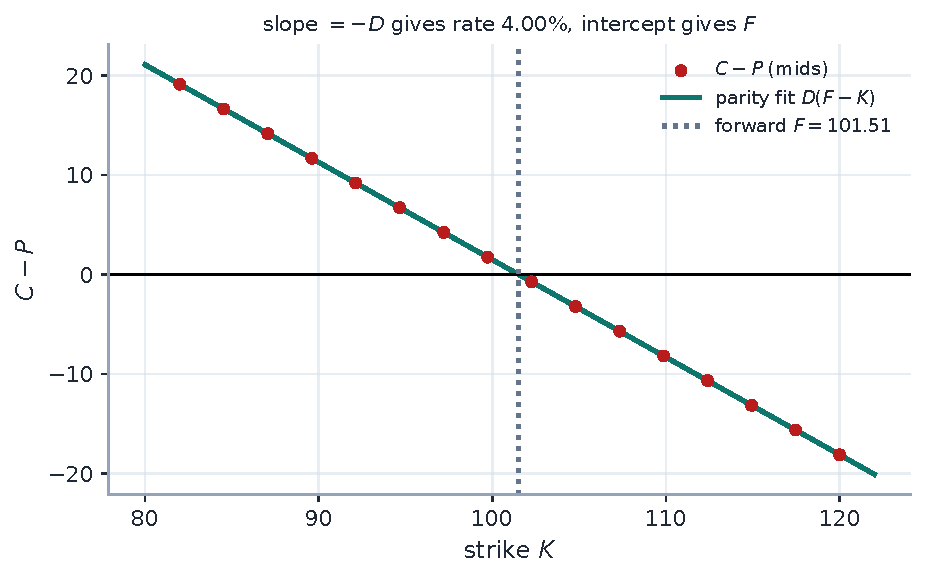
\includegraphics[width=0.74\textwidth]{fig_fwd_parity.pdf}
\caption{The put--call parity regression $C-P=D(F-K)$. The slope is the discount
($\to$ rate $\fwdrate\%$), the intercept gives the forward ($F=\fwdhat$, true
$\fwdtrue$).}
\label{fig:parity}
\end{figure}

%======================================================================
\section{The discount clamp}
\label{sec:clamp}

The parity slope \emph{is} the discount, and it is the worst-identified parameter
in \eqref{eq:regress}: the price difference $C-P$ changes slowly with strike, so a
little noise in the mids tilts the line a lot. On a clean chain this is harmless; on
a noisy or stale delayed feed it drifts to nonsense --- an implied discount $D>1$,
i.e.\ a \emph{negative} rate, which tilts the forward and gaps the ATM smile.

\begin{caution}
A negative implied rate is not a market signal here; it is feed noise in the least
reliable regression parameter. Letting it through propagates a small price error
into a large level error: a $5\%$ discount error shifts the whole implied-vol level.
The forward's \emph{level} (the intercept) is well identified; its \emph{slope}
(the discount) is not.
\end{caution}

The fix, when a reference date pins the year fraction, is to clamp the
parity-implied rate $r=-\log D/T$ to a physical band
$[\text{\fwdratemin}\%,\text{\fwdratemax}\%]$. Clean chains sit strictly inside the
band and are byte-identical. When the clamp bites, the forward is \emph{re-derived
from the well-identified price level} at the clamped discount --- a per-strike
average of $K+(C-P)/D$ weighted by quote quality (tighter spreads and
near-ATM strikes count more, kernel width $0.10$ in log-moneyness) --- rather
than from the tilted slope. So the robust forward keeps the good information
(the level) and discards the bad (the runaway slope). A final sanity bound
$|\log(F/S)|<\text{FWD\_CLAMP\_LOG}=0.5$ falls back to spot if even the level
is unusable. \Cref{fig:clamp} shows the implied rate leaving the band as the
slope is perturbed and the clamp pinning it.

\begin{example}[title={Case file: the delayed feed that gapped the ATM smile}]
\textbf{Setup.} Live SPY on the Massive delayed feed; also reproduced on a
Bloomberg fixture. Quotes are individually sane but collectively stale ---
mids drift asynchronously across strikes.

\textbf{Failure mode.} The parity regression returned discounts of
$1.01$--$1.015$ live (up to $1.024$ on the fixture): an implied \emph{negative}
rate. The tilted slope dragged the forward, and every ATM smile showed the
telltale gap between the put and call sides.

\textbf{The failed first fix.} Anchoring the \emph{rate} per expiry to a
smoothed term structure looked principled --- and broke everything: the
per-expiry discounts came out jagged, the LV benchmark regressed, and the
attempt deadlocked \texttt{state.forwards}. Reverted. The lesson: do not
repair the ill-identified parameter by making it a fitted object with even
more structure; \emph{stop trusting it}.

\textbf{Fix.} The clamp above: pin the rate to the physical band, re-derive
the forward from the quality-weighted price level, keep spot as the last
resort. The discount stays exactly what parity gave whenever it is physical.

\textbf{Verdict (test-locked).} Clean chains recovered to truth and
unclamped (byte-identical); stale-wing chains that break the unclamped
regression stay sane under the clamp; zero-spread close-like data still
resolves; and with no reference date (year fraction unknown) the clamp
correctly stands down. The residual ATM jitter that remains on the delayed
feed is feed noise, not the forward.
\end{example}

\begin{figure}[H]
\centering
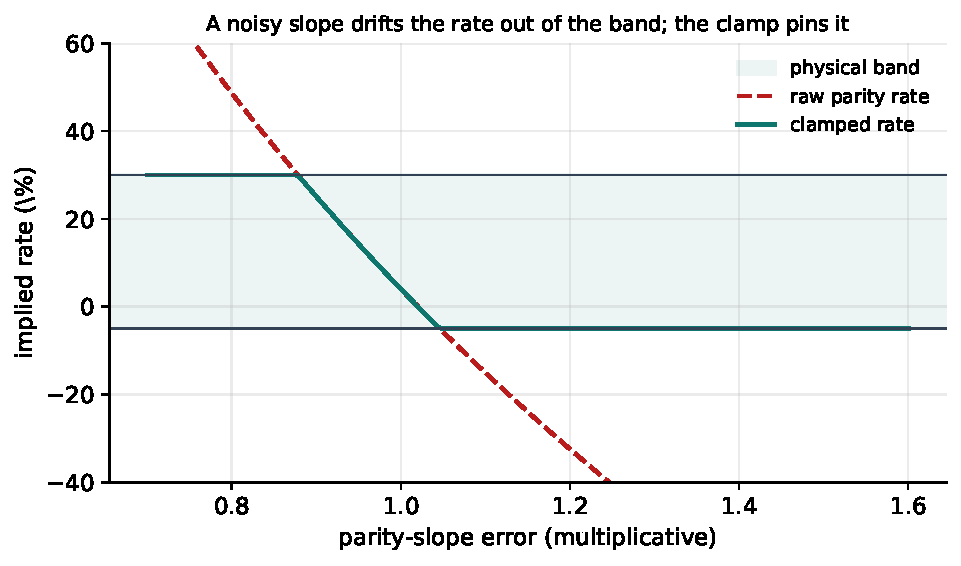
\includegraphics[width=0.74\textwidth]{fig_fwd_clamp.pdf}
\caption{As a multiplicative slope error perturbs the discount, the raw parity rate
(dashed) leaves the physical band; the clamp (solid) pins it to
$[\fwdratemin\%,\fwdratemax\%]$ and the forward is re-derived from the price level.}
\label{fig:clamp}
\end{figure}

The clamp bounds an \emph{absurd} answer. There is one failure mode it cannot
see: a chain whose parity content is exactly zero, where the regression returns
a wrong answer that is perfectly \emph{plausible}. That case needs its own
device.

%======================================================================
\section{The zero-carry pin}
\label{sec:zerocarry}

Delayed data tiers can gate the live quote stream (the NBBO). When that
happens, a provider does not return an empty chain --- it \emph{synthesizes}
one from its per-contract implied vols, pricing every contract with Black at
$F=S$, $D=1$, and quoting it with zero spread
(\texttt{data/massive.py}). Those prices are perfectly self-consistent, but
they contain \emph{no} put--call parity information: the forward and discount
were not observed, they were \emph{assumed} by the synthesis. Worse, the
provider's call and put IVs embed the provider's \emph{own} carry model, so
once its contracts are re-priced at zero carry the call/put asymmetry survives
in the prices --- and a parity regression dutifully reads that asymmetry as a
forward and a discount that nobody ever quoted.

\begin{example}[title={Case file: the garbage forwards the clamp could not see}]
\textbf{Setup.} Live SPY on the Massive delayed tier, recurring over several
sessions: the tier gated the NBBO quotes, so every chain the app received was
IV-synthesized at zero carry.

\textbf{Failure mode.} Recurring garbage forwards on a healthy-looking feed:
short-dated implied rates of $-3.8\%$, discounts above one, and a one-year
forward $+1.7\%$ \emph{above} the $F=S$ the prices had been built with. The
discount clamp of \cref{sec:clamp} stayed silent throughout --- the spurious
rates sat \emph{inside} the physical band, so there was nothing absurd to
bound. (The same saga's failed first fix --- anchoring the rate to a smoothed
term structure --- is the one described in \cref{sec:clamp}: it regressed the
LV benchmark and deadlocked the forwards state before being reverted.)

\textbf{Diagnosis.} The regression was not noisy; it was answering a question
the data could not ask. Every synthesized price is Black at $F=S$, $D=1$, so
the only structure left for the regression to find is the provider's call/put
IV asymmetry --- a spurious signal that is \emph{small enough to be
plausible}, which is exactly why the clamp (built for absurd slopes) never
fired.

\textbf{Fix.} Recognize the regime at ingestion, not in the regression. The
provider layer flags the synthesized snapshot
(\texttt{ChainSnapshot.zero\_carry} in \texttt{data/types.py}); for a flagged
chain \texttt{implied\_forward} returns the chain's own construction
convention --- $F=S$, $D=1$, zero residual --- and never regresses. The flag
is \emph{explicit} and persists with the snapshot (store schema v5), so
captured chains replay correctly; it is deliberately \emph{not} inferred from
chain-wide zero spreads, because EOD close marks also quote
$\text{bid}=\text{ask}$ yet their mids carry genuine parity information. The
Forwards tab shows a badge (``IV-synthesized $\cdot$ zero carry $\cdot$ $F$
pinned to spot'') so the desk knows the forward is a convention, not a market
read.

\textbf{Verdict (test-locked).} A flagged zero-carry chain pins to $F=S$,
$D=1$ on both the reference-date and legacy paths (the flag, not the clamp,
decides); an \emph{unflagged} zero-spread chain still regresses and recovers
its true carry; the flag round-trips through the store. The recurring SPY
forward incident is closed at the root.
\end{example}

The pin completes an epistemic ladder: the regression extracts the forward
where parity is informative; the clamp refuses the slope where parity is
noisy; and the pin refuses the regression entirely where parity is
\emph{vacuous} --- returning the only honest answer the chain contains, its
own construction convention. The regime matters downstream too: on such feeds
anything that needs a carry (the de-Americanization of Note~05, for instance)
must source it externally, because the parity-implied carry is not merely
noisy but meaningless.

%======================================================================
\section{Dividends}
\label{sec:divs}

The carry that links spot to forward, $F=S\,e^{(r-q)T}$, must account for
dividends. Four modes coexist (Note~05 uses the same machinery for the pricing
tree):
\begin{itemize}[leftmargin=1.4em]
\item \textbf{Discrete cash} (\texttt{discrete\_absolute}): a schedule of ex-dates
and cash amounts, priced by the escrowed-spot method ---
$F=(S-\sum_iD_ie^{-r\tau_i})\,e^{rT}$ --- with early exercise evaluated
against the actual cum-dividend spot.
\item \textbf{Discrete proportional} (\texttt{discrete\_proportional}): ex-date
percentage haircuts, for names that quote dividends as yields per event.
\item \textbf{Continuous yield} (\texttt{continuous}): a constant $q$, a crude but
cheap proxy for far-dated proportional dividends.
\item \textbf{Mixed} (\texttt{mixed}): discrete cash for near ex-dates,
switching to a proportional/continuous tail beyond a horizon
(\texttt{switch\_years}) --- the realistic single-name default shape.
\end{itemize}
The dividend mode is per ticker and editable; it feeds both the forward carry
and the de-Americanization tree, and an equivalent-yield round trip across all
four modes is test-locked.

%======================================================================
\section{American de-bias}
\label{sec:debias}

There is a circularity between the forward and de-Americanization: the forward sets
the carry $q$, the carry drives early exercise, and de-Americanizing the puts and
calls re-implies the forward. The raw parity regression uses American mids
directly, which biases the forward slightly because the early-exercise premium is
not symmetric between puts and calls. The \emph{de-bias} resolves this with the
discount \emph{held}: fixing the rate $r=-\log D/T$ from the raw parity, each round
sets the carry $q=r-\log(F/S)/T$ from the current forward, de-Americanizes the
near-ATM call and put mids to European-equivalent Black vols, reprices them as
European, and re-implies the forward at the \emph{fixed} slope $-D$,
\begin{equation}
F\ \leftarrow\ \frac{1}{D}\,\overline{\big(y+D\,K\big)},\qquad y=\text{European }(C-P),
\end{equation}
iterating to the fixed point where the two de-Americanized OTM sides join. Only a
near-ATM band of strikes and a coarse tree enter --- it locates the forward to
$\sim1$ basis point in a few milliseconds, while quote prep does the
full-precision per-quote de-Americanization downstream. The discount is left
exactly as the raw parity gave it.

%======================================================================
\section{What is original here}
\label{sec:original}

Parity forward extraction is textbook; the robustness engineering is the
contribution. The \emph{discount clamp} encodes the right epistemics --- trust the
well-identified price level, distrust the ill-identified slope, and re-derive the
forward accordingly --- so the app survives the noisy delayed feeds that would
otherwise gap every ATM smile. The \emph{zero-carry pin} extends the same
epistemics to the degenerate case: a synthesized chain carries no parity
information at all, so the honest forward is the chain's own construction
convention, recognized by an explicit ingestion-time flag rather than any
inference from the prices. The \emph{de-bias} closes the forward/de-Am
circularity at the fixed point that quote prep actually uses, with the discount
held so the two corrections do not fight. All three are byte-identical on clean
data, so the robustness costs nothing when it is not needed.

%======================================================================
\section{Traceability}
\label{sec:traceability}

\begingroup
\small
\setlength{\tabcolsep}{3pt}
\begin{longtable}{@{}p{0.32\textwidth}p{0.11\textwidth}p{0.25\textwidth}p{0.28\textwidth}@{}}
\caption{Claims in this note and the code/tests that lock them.}\\
\toprule Claim & Object & Code anchor & Test anchor\\ \midrule
\endfirsthead
\toprule Claim & Object & Code anchor & Test anchor\\ \midrule
\endhead
Clean chain: truth recovered, clamp inert (byte-identical) &
\cref{sec:clamp} &
\nolinkurl{data/forwards.py} &
\nolinkurl{test_forward_robust.py::test_clean_chain_recovered_to_truth_and_unclamped}\\
Stale wings break the raw regression; clamp stays sane &
case file &
\nolinkurl{data/forwards.py} &
\nolinkurl{test_forward_robust.py::test_stale_wings_break_unclamped_but_clamp_stays_sane}\\
No reference date $\Rightarrow$ clamp stands down &
\cref{sec:clamp} &
\nolinkurl{data/forwards.py} &
\nolinkurl{test_forward_robust.py::test_no_reference_date_skips_clamp}\\
Zero-carry chain pinned to $F=S$, $D=1$ (flag decides, both paths) &
\cref{sec:zerocarry} &
\nolinkurl{data/forwards.py}, \nolinkurl{data/types.py} &
\nolinkurl{test_forward_robust.py::test_zero_carry_chain_pins_forward_to_spot}\\
Zero spreads alone never trigger the pin &
invariant~4 &
\nolinkurl{data/types.py} (\nolinkurl{is_zero_carry}) &
\nolinkurl{test_forward_robust.py::test_unflagged_zero_spread_chain_still_regresses}\\
Provider flags synthesized chains; flag persists (schema v5) &
\cref{sec:zerocarry} &
\nolinkurl{data/massive.py}, \nolinkurl{data/store.py} &
\nolinkurl{test_massive.py::test_iv_fallback_synthesizes_fittable_chain}, \nolinkurl{test_data_layer.py::test_snapshot_round_trip_keeps_zero_carry}\\
De-bias holds the discount, smooths the forward &
\cref{sec:debias} &
\nolinkurl{data/forwards.py} (\nolinkurl{_refine_american}) &
\nolinkurl{test_forward_debias.py::test_debias_holds_discount_debiases_forward_and_smooths}\\
No localized ATM spike after de-bias &
\cref{sec:why} &
\nolinkurl{data/forwards.py} &
\nolinkurl{test_forward_debias.py::test_debiased_smile_has_no_localized_atm_spike}\\
European chains unaffected by the de-bias &
\cref{sec:debias} &
\nolinkurl{data/forwards.py} &
\nolinkurl{test_forward_debias.py::test_european_chain_unaffected_by_reference_date}\\
All four dividend modes; equivalent-yield round trip &
\cref{sec:divs} &
\nolinkurl{data/dividends.py} &
\nolinkurl{test_dividends.py::test_equivalent_yield_round_trips_every_mode}, \nolinkurl{::test_mixed_forward_switches_at_horizon}\\
Per-ticker forwards version scoping &
invariant~5 &
\nolinkurl{api/state.py} &
\nolinkurl{test_api_forwards.py::test_parity_defaults_cover_the_ladder}\\
\bottomrule
\end{longtable}
\endgroup

\appendix
%======================================================================
\section{Hyperparameter atlas}
\label{app:atlas}

\begin{longtable}{p{0.27\textwidth}p{0.16\textwidth}p{0.49\textwidth}}
\caption{Forward/dividend hyperparameters.}\label{tab:atlas}\\
\toprule Knob & Default & Role\\ \midrule
\endfirsthead \toprule Knob & Default & Role\\ \midrule \endhead
\multicolumn{3}{l}{\emph{Surfaced}}\\ \midrule
\texttt{ForwardPolicy.mode} & \texttt{parity} & \texttt{parity} (regression) or \texttt{theoretical} (carry model).\\
\texttt{MarketSettings.rate} $r$ & --- & Risk-free rate for the theoretical forward / tree.\\
\texttt{dividendMode} & \texttt{continuous} & \texttt{continuous} yield or \texttt{discrete\_absolute} cash.\\
\texttt{dividends} & empty & Discrete $(\text{ex-date},\text{amount})$ schedule.\\
\midrule
\multicolumn{3}{l}{\emph{Hidden}}\\ \midrule
\texttt{RATE\_MIN/MAX} & $[\fwdratemin\%,\fwdratemax\%]$ & Physical band for the parity-implied rate (clamp).\\
\texttt{FWD\_CLAMP\_LOG} & $0.5$ & Sanity bound on $|\log(F/S)|$; else fall back to spot.\\
\texttt{MIN\_PAIRED\_STRIKES} & $3$ & Minimum paired strikes for a parity fit.\\
\texttt{OUTLIER\_NSIGMA} / \texttt{MAX\_TRIM\_ROUNDS} & $4$ / $3$ & Residual
trim threshold and iteration cap in the parity fit.\\
\texttt{ATM\_KERNEL\_H} & $0.10$ & ATM Gaussian kernel width in the
level-re-derivation quality weights.\\
\texttt{DEAM\_REFINE\_BAND} & $0.15$ & Log-moneyness band entering the de-bias
iteration.\\
\texttt{MAX\_DEAM\_ITERS} & $6$ & De-bias fixed-point iterations.\\
\bottomrule
\end{longtable}

\noindent\textbf{Performance.} The parity regression is a $2\times2$ least squares
per expiry; the clamp is a comparison; the de-bias is a handful of coarse-tree
de-Americalizations on a near-ATM band ($\sim1$ bp forward in a few ms). All are
negligible against the smile fit, and editing a name's rate or dividend schedule
bumps only that ticker's forwards version, refitting just that name.

%======================================================================
\section{Reference implementation: the discount clamp}
\label{app:ref}

The parity \emph{slope} is the discount --- the worst-identified parameter --- so on
a noisy feed it can imply a nonphysical rate. The clamp pins the rate to a band and,
when it bites, re-derives the forward as a per-strike average $F=\operatorname{mean}
(K+(C-P)/D)$ (the well-identified \emph{level}) rather than the slope-driven $a/b$,
so the forward no longer inherits the bad slope.

\begin{lstlisting}[caption={The discount clamp and forward re-derivation ---
simplified from \texttt{data/forwards.py}, where the clamp is inline in
\texttt{implied\_forward} and the level mean is the quality-weighted
\texttt{\_forward\_at\_discount} (spread $\times$ ATM kernel), with the spot
fallback of \cref{sec:clamp}.}]
def clamp_forward(K, call_mid, put_mid, t, F, D, r_lo=-0.05, r_hi=0.30):
    r = -np.log(D)/t                     # the parity discount's implied rate
    if r_lo <= r <= r_hi:
        return F, D                      # physical: keep the regression result
    D = np.exp(-np.clip(r, r_lo, r_hi)*t)         # clamp the rate to the band
    F = np.mean(K + (call_mid - put_mid)/D)       # re-derive F from the LEVEL, not a/b
    return F, D
\end{lstlisting}

\begin{thebibliography}{9}
\bibitem{Hull2017} J.~Hull. \emph{Options, Futures, and Other Derivatives}.
Pearson, 10th ed., 2017.
\bibitem{Gatheral2006} J.~Gatheral. \emph{The Volatility Surface}. Wiley, 2006.
\end{thebibliography}

\end{document}
